%%%%%%%%%%%%%%%%%%%%%%%%%%%%%%%%%%%%%
%                                   %
% Compile with XeLaTeX and biber    %
%                                   %
% Questions or comments:            %
%                                   %
% joshua dot mcneill at uga dot edu %
%                                   %
%%%%%%%%%%%%%%%%%%%%%%%%%%%%%%%%%%%%%

\documentclass{beamer}
  % Read in standard preamble (cosmetic stuff)
  %%%%%%%%%%%%%%%%%%%%%%%%%%%%%%%%%%%%%%%%%%%%%%%%%%%%%%%%%%%%%%%%
% This is a standard preamble used in for all slide documents. %
% It basically contains cosmetic settings.                     %
%                                                              %
% Joshua McNeill                                               %
% joshua dot mcneill at uga dot edu                            %
%%%%%%%%%%%%%%%%%%%%%%%%%%%%%%%%%%%%%%%%%%%%%%%%%%%%%%%%%%%%%%%%

% Beamer settings
% \usetheme{Berkeley}
\usetheme{CambridgeUS}
% \usecolortheme{dove}
% \usecolortheme{rose}
\usecolortheme{seagull}
\usefonttheme{professionalfonts}
\usefonttheme{serif}
\setbeamertemplate{bibliography item}{}

% Packages and settings
\usepackage{fontspec}
  \setmainfont{Charis SIL}
\usepackage{hyperref}
  \hypersetup{colorlinks=true,
              allcolors=blue}
\usepackage{graphicx}
  \graphicspath{{../../figures/}}
\usepackage[normalem]{ulem}
\usepackage{enumerate}

% Document information
\author{M. McNeill}
\title[FREN2001]{Français 2001}
\institute{\url{joshua.mcneill@uga.edu}}
\date{}

%% Custom commands
% Lexical items
\newcommand{\lexi}[1]{\textit{#1}}
% Gloss
\newcommand{\gloss}[1]{`#1'}
\newcommand{\tinygloss}[1]{{\tiny`#1'}}
% Orthographic representations
\newcommand{\orth}[1]{$\langle$#1$\rangle$}
% Utterances (pragmatics)
\newcommand{\uttr}[1]{`#1'}
% Sentences (pragmatics)
\newcommand{\sent}[1]{\textit{#1}}
% Base dir for definitions
\newcommand{\defs}{../definitions}


  % Packages and settings

  % Document information
  \subtitle[Prépositions et verbes \lexi{-re}]{Les prépositions de lieu et les verbes \lexi{-re}}

\begin{document}
  % Read in the standard intro slides (title page and table of contents)
  \begin{frame}
    \titlepage
    \tiny{Office: % Basically a variable for office hours location
Gilbert 121\\
          Office hours: % Basically a variable for office hours
 lundi, mercredi, vendredi 10:10--11:10
}
  \end{frame}

  \begin{frame}{Annonces}
    \begin{itemize}
      \item
      \item[] \tinygloss{}
    \end{itemize}
  \end{frame}

  \begin{frame}{Les verbes \lexi{-re}}
    \begin{center}
      \begin{tabular}{l | l l | l l}
  \multicolumn{5}{c}{attendre \gloss{to wait}} \\
      & \multicolumn{2}{l |}{singulier} & \multicolumn{2}{l}{pluriel} \\
  \hline
  1re & j'         & attends            & nous        & attendons \\
  2e  & tu         & attends            & vous        & attendez \\
  \hline
  3e  & il (masc)  &                    & ils (masc)  & \\
      & elle (fem) & attend             & elles (fem) & attendent \\
      & on         &                    &             & \\
\end{tabular}

    \end{center}
  \end{frame}

  \begin{frame}{Les prépositions de lieu}
    \begin{columns}
      \column{0.5\textwidth}
        % Use a map of downtown Athens
        \begin{enumerate}
          \item
        \end{enumerate}
      \column{0.5\textwidth}
        \begin{minipage}[c][0.6\textheight]{\linewidth}
          \begin{center}
            \only<1-2>{
              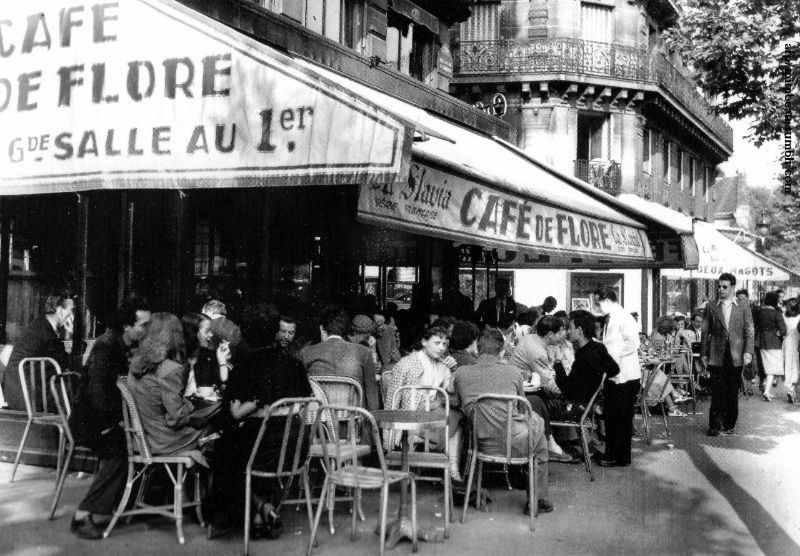
\includegraphics[scale=0.2]{cafe.jpg}
            }
          \end{center}
        \end{minipage}
    \end{columns}
  \end{frame}

  \begin{frame}{}
    \begin{center}
      \Large Quiz
    \end{center}
  \end{frame}

  \begin{frame}{Réponses personnelles}
    Pose les questions suivantes à un/e partenaire. \\
    \tinygloss{Ask a partner the following questions.}
    \begin{center}
      \begin{enumerate}
        \item À qui est-ce que tu rends visite le week-end?
        \item Est-ce que tu perds souvent tes affaires \gloss{things}? Si oui, comment?
        \item Est-ce que tu vends tes livres de cours à la fin du semestre? Pourquoi?
        \item Est-ce que tu réponds rapidement aux textos? Pourquoi?
        \item Quand est-ce que tu descends en ville, et pourquoi?
      \end{enumerate}
    \end{center}
  \end{frame}

  \begin{frame}{Sur le campus}
    Choisis un endroit sur le campus, puis circule dans la salle pour demander à tes camarades de classe où cet endroit se trouve.
    Fais des notes des différentes façons de décrire sa disposition. \\
    \tinygloss{Choose a place on campus, then go around the room to ask your classmates where this place is located.
    Take note of the different ways to discribe its position.} \\
    \begin{center}
      \begin{description}
        \item[] \textbf{Modèle:}
        \item[E1:] C'est où, la cafétéria Bolton?
        \item[E2:] C'est en face du MLC.
        \item[E3:] C'est près de Sanford Hall.
      \end{description}
    \end{center}
    \begin{columns}
      \column{0.5\textwidth}
        \begin{enumerate}
          \item la bibliothèque
          \item le centre étudiant
          \item la piscine
          \item le bureau des inscriptions
        \end{enumerate}
      \column{0.5\textwidth}
        \begin{enumerate}
          \setcounter{enumi}{4}
          \item le théâtre
          \item la librairie
          \item la cafétéria
          \item les terrains de sport
        \end{enumerate}
    \end{columns}
  \end{frame}

  \begin{frame}{}
    \begin{center}
      \Large Questions?
    \end{center}
  \end{frame}
\end{document}
